\documentclass[a4paper,12pt]{article}
\usepackage[style=authoryear,sorting=ynt, maxbibnames=2]{biblatex}
\usepackage[unicode, draft=false]{hyperref}
\usepackage[scale=0.9]{geometry}
\usepackage{xcolor}
\usepackage{graphicx}
\usepackage{amsmath}

\title{Teleprocessamento e Redes - Relatório do trabalho final}
\author{
  Leonardo Ribeiro Santiago (120036072) \\
  João Matheus Nascimento Gonçalves (120023786) \\
  Esteves Emmanuel Melo Ferreira (117209640) }

\newcommand{\code}[1]{\texttt{#1}}

\date{}

\begin{document}

\maketitle

\section{Introdução}

Neste relatório iremos responder as perguntas relacionadas à parte 2 do trabalho final. O código está disponível no seguinte repositório do github: {\color{blue} \href{https://github.com/o-santi/redes}{github.com/o-santi/redes}}.

Para reproduzir os resultados, deve-se instanciar uma máquina virtual Ubuntu usando Vagrant, assim como descrito em {\color{blue} \href{https://github.com/kaichengyan/mininet-vagrant}{github.com/kaichengyan/mininet-vagrant}}. Uma vez dentro da VM, clonamos o repositório git para uma pasta interna, e rodamos o arquivo \code{run.sh}.
\begin{verbatim}
  git clone -b entrega-preliminar https://github.com/o-santi/redes.git ~/redes
  cd ~/redes/bufferbloat
  chmod +x ./run.sh
  sudo ./run.sh
\end{verbatim}

Isto irá rodar os dois casos de teste (\code{max\_queue=20} e \code{max\_queue=100}) e gerar os gráficos citados neste relatório.

\section{Parte 2}

\subsection{Qual é o tempo médio de busca da página da web e seu desvio padrão quando q=20 e q=100?}

No caso \code{q=20}, o tempo médio de busca da página é de 3,30 segundos, com um desvio padrão de 0,82.
\begin{figure}[h!]
  \centering
  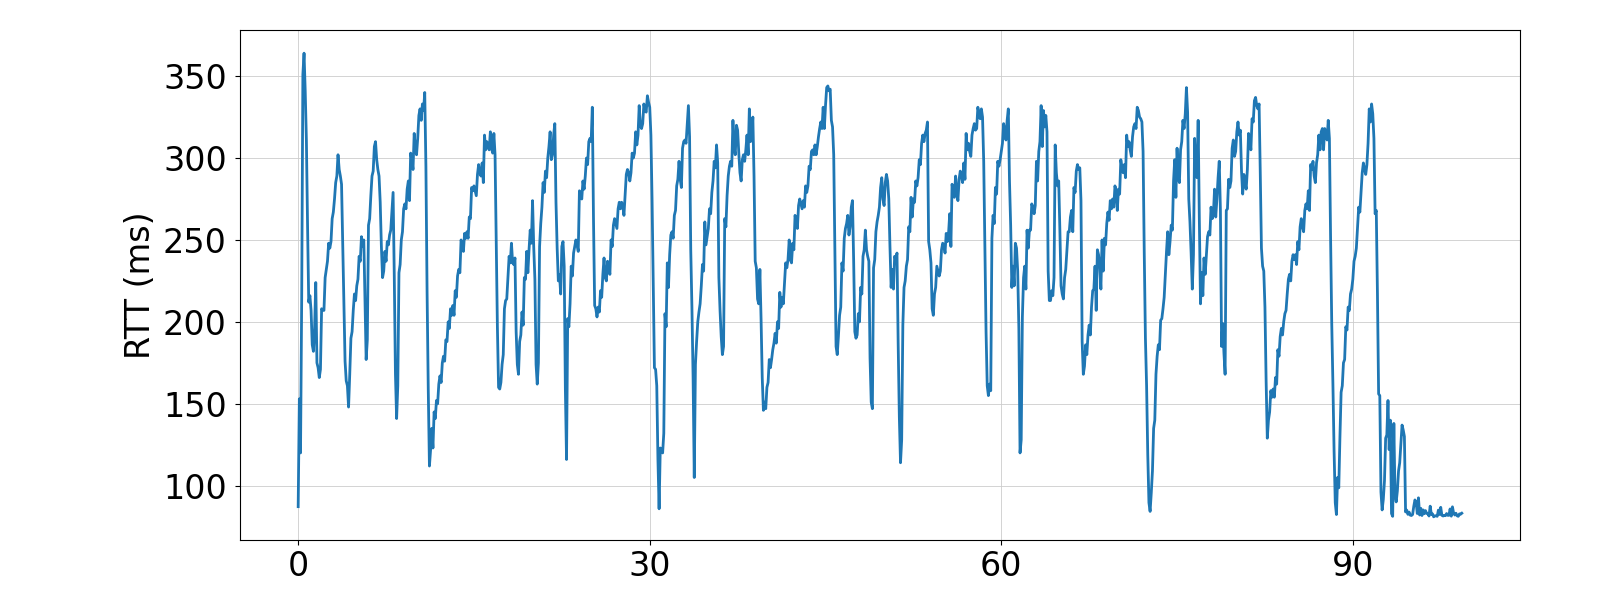
\includegraphics[width=0.5\columnwidth]{./bufferbloat/reno-rtt-q20.png}
  \caption{Tempo de resposta dos pings ao longo da duração do teste.}
  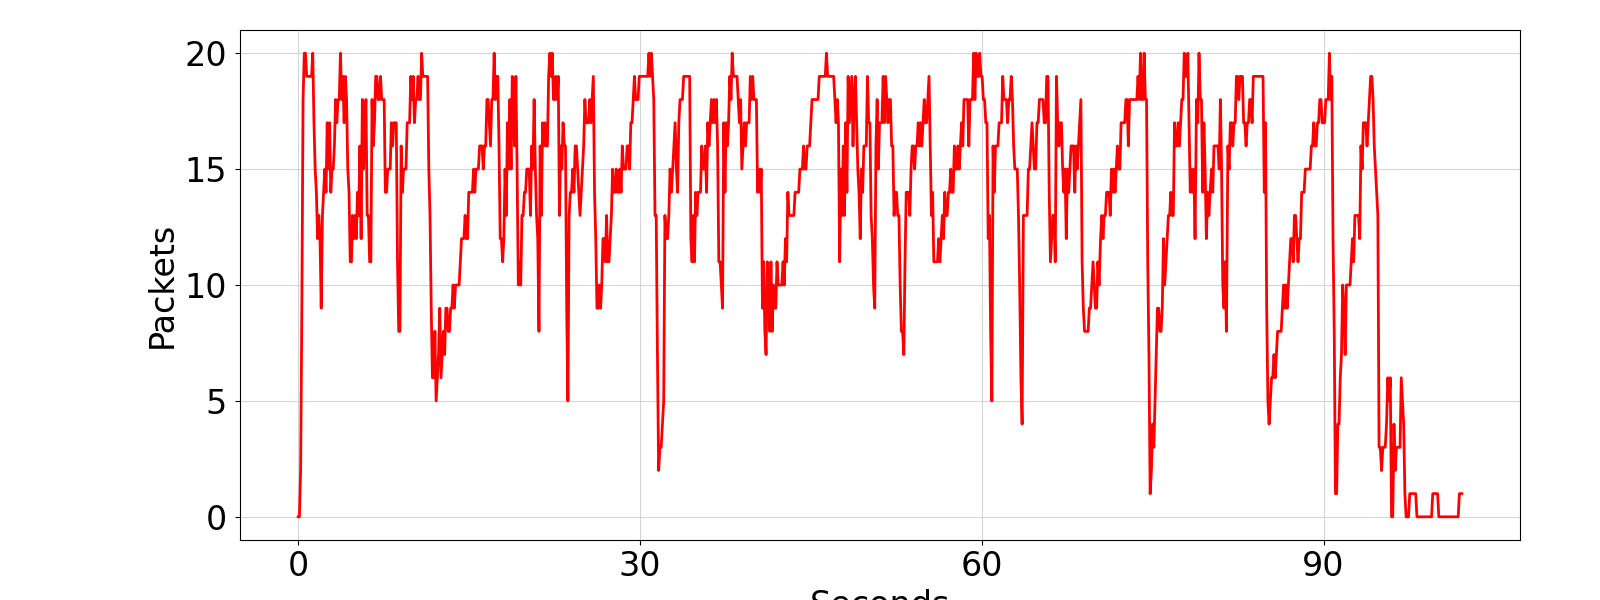
\includegraphics[width=0.5\columnwidth]{./bufferbloat/reno-buffer-q20.png}
  \caption{Número de pacotes na fila do switch ao longo do teste.}
\end{figure}

\newpage

Já no caso \code{q=100}, o tempo médio é de 9,96 segundos, com um desvio padrão de 3,17.

\begin{figure}[h!]
  \centering
  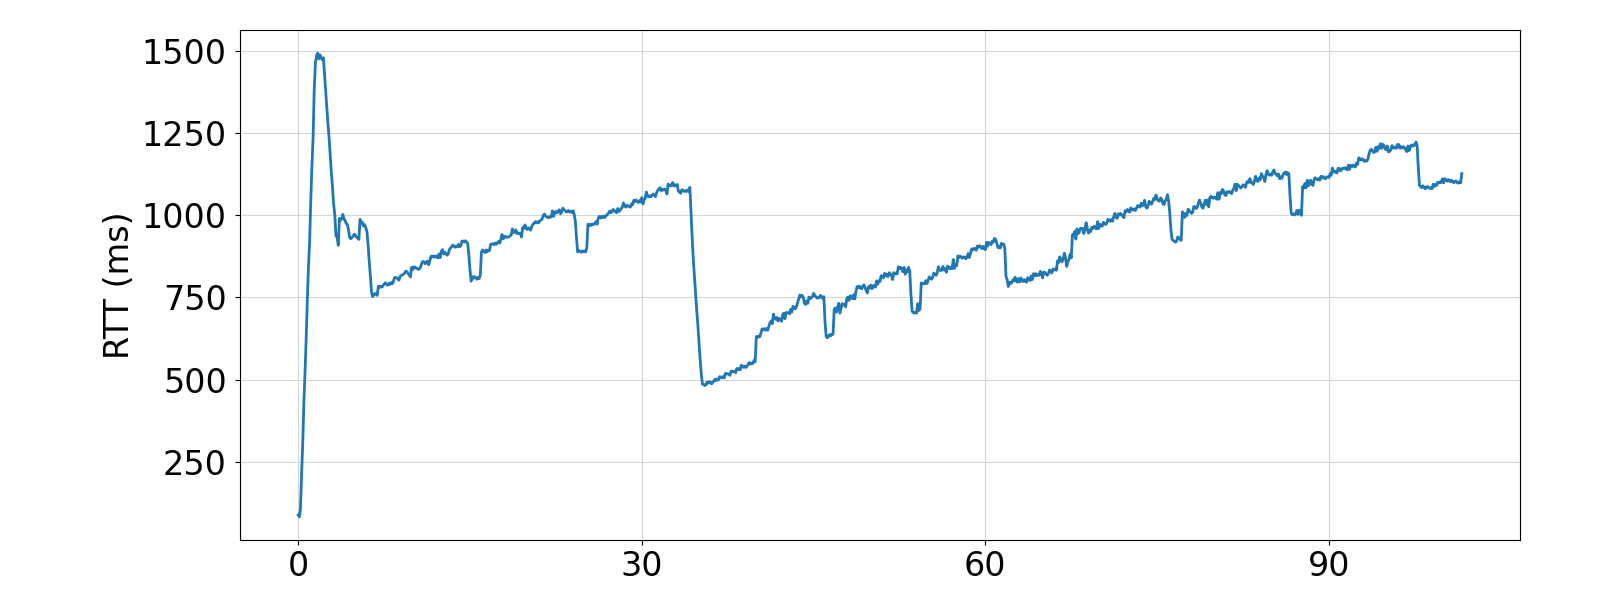
\includegraphics[width=0.5\columnwidth]{./bufferbloat/reno-rtt-q100.png}
  \caption{Tempo de resposta dos pings ao longo da duração do teste.}
  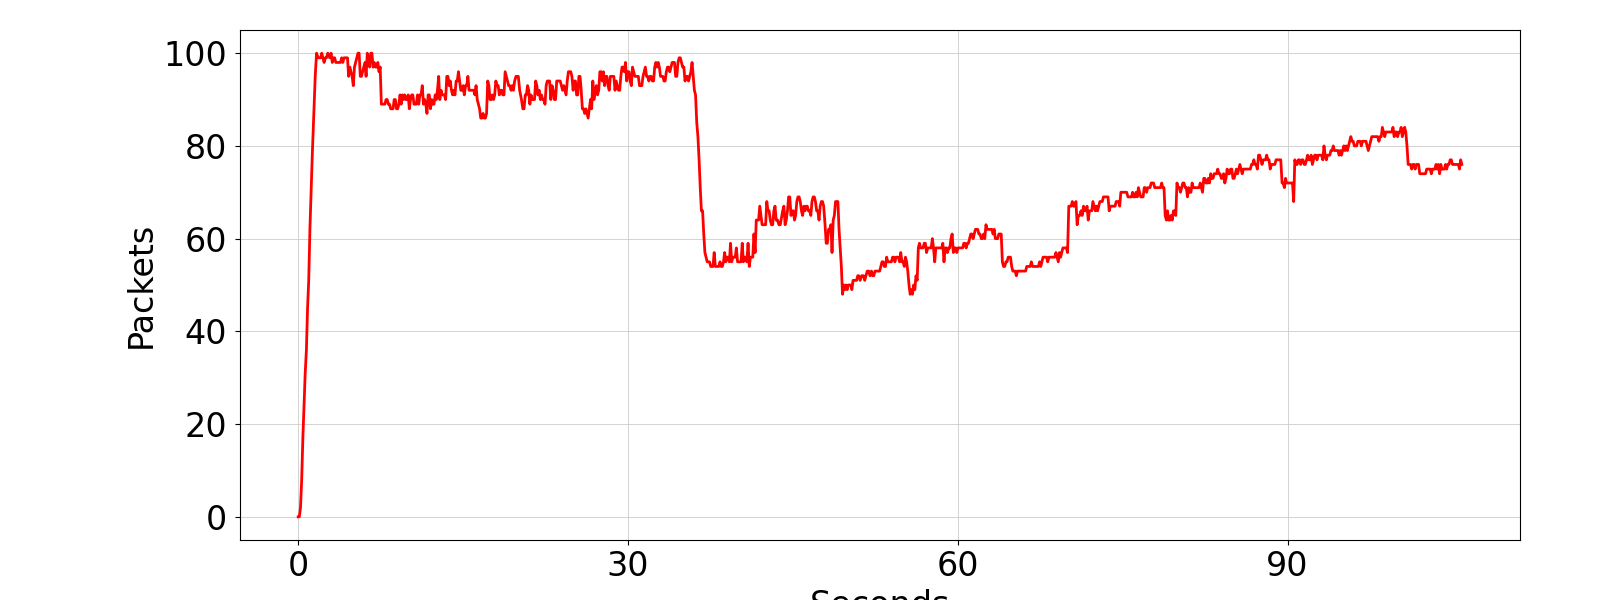
\includegraphics[width=0.5\columnwidth]{./bufferbloat/reno-buffer-q100.png}
  \caption{Número de pacotes na fila do switch ao longo do teste.}
\end{figure}

\subsection{Por que você vê uma diferença nos tempos de busca de páginas da Web com buffers de roteador curtos e grandes?}

A diferença pode ser explicada pela maior quantidade de pacotes que entram na fila, fazendo com que a janela de congestão da conexão TCP aumente, fazendo com que os pacotes passem mais tempo na fila esperando para serem transmitidos.

Ao diminuir o tamanho da fila para 20, os pacotes param de acumular como antes, fazendo com que o tempo que um pacote deve esperar na fila seja reduzido.

\subsection{Bufferbloat pode ocorrer em outros lugares, como sua placa de interface de rede (NIC). Verifique a saída de ifconfig eth0 de sua VM mininet. Qual é o comprimento (máximo) da fila de transmissão na interface de rede relatada pelo ifconfig? Para esse tamanho de fila, se você assumir que a fila é “drenada” a 100 Mb/s, qual é o tempo máximo que um pacote pode esperar na fila antes de sair da NIC?
}

Rodando \code{h1 ifconfig} de dentro da mininet, vemos que o parâmetro \code{txqueuelen} da interface principal \code{h1-eth0} é de 1000 pacotes, com \code{mtu=1500 bytes}.

Isso significa que, se um pacote entrar na última posição da fila, ele deve esperar todos os 999 pacotes transmitirem, e depois esperar o tempo da sua própria transmissão. O tempo máximo de transmissão de um pacote, na velocidade de \code{100Mb/s} é de $\frac{1000 * 1500 * 8}{100.000.000} \text{ segundos} = \frac{15 * 8}{1000} \text{ segundos} \approx 0,12 \text{ segundos} $. 

\subsection{Como o RTT relatado pelo ping varia com o tamanho da fila? Descreva a relação entre os dois.}

Tanto no caso \code{q=20} quanto quando \code{q=100}, o \code{RTT} aumenta linearmente com o número de pacotes na fila. Isso se dá pois o tempo de transmissão na rede é constante, dado que o único gargalo é o switch principal. Assim, quanto mais pacotes na fila do switch, maior será o tempo que ele levará para ser transmitido, e portanto maior será o RTT.

\subsection{Identifique e descreva duas maneiras de mitigar o problema de bufferbloat.}

De modo geral, técnicas para mitigar o \textit{bufferbloat} podem ser separadas em duas categorias: as que visam melhorar a rede e as que visam melhorar as pontas da conexão.

Dos que visam melhorar a rede, vale ressaltar os algorítmos \code{CoDel} (\textit{Controled Delay}) e sua melhoria \code{FQ-Codel} (\textit{Fair/Flow Queue CoDel}), que está dentro da categoria de algoritmos de \textit{Active Queue Management} (\code{AQM}). Esse algoritmo busca controlar o limite do delay que os pacotes experienciam nas filas dos roteadores para um máximo de 5 millisegundos. Caso o número de pacotes aumente rapidamente, de forma que o delay passe desse \textit{threshold}, pacotes são descartados da fila até que o delay esteja dentro do limite aceitável.

Dos que visam melhorar as pontas da conexão, destaca-se uma implementação do protocolo TCP utilizando um algoritmo de congestão diferente do \code{Reno}: o \textit{Bottleneck Bandwidth and Round-trip propagation time} (\code{BBR}). Diferentemente do \code{Reno}, que utiliza a perda de pacotes para detectar congestionamento e baixas taixas de transmissão, o \code{BBR} constroi um modelo da rede, utilizandos amostras de pacotes para medir a taxa de transmissão e o \textit{Round Trip Time} (\code{RTT}).

%% \section{Parte 3}


\end{document}
